%!TEX root = ../../../tugas-akhir.tex

\section{Rancangan Paralelisasi}
  \subsection{Implementasi Komputasi Paralel} \label{sec:parallel_env}

    % Jelasin MPI, OpenMP, POSIX. Kelebihan, kekurangan, mana yang cocok dipake.
    % Terdapat beberapa kakas yang dapat dimanfaatkan untuk menjalankan komputasi paralel dalam sebuah program.
    Dalam implementasi komputasi paralel dalam bahasa C, terdapat tiga kakas yang umum digunakan yaitu POSIX threads, OpenMP, dan MPI. Setiap kakas tersebut memiliki kelebihan dan kekurangan yang berbeda. Setiap kakas memiliki usecase khusus dimana penggunaannya akan menghasilkan kinerja yang baik dan implementasi komputasi paralel dapat dilakukan dengan relatif mudah.

    % Kasih usecase buat tiap model
    % jelasin thread, kekurangan ribet serba manual, kelebihan sudah native, ga nambah overhead banyak, relatif sederhana
    POSIX threads (pthread) adalah sebuah model eksekusi dalam komputasi paralel yang dimiliki sistem operasi UNIX secara native. POSIX thread merupakan sebuah implementasi shared memory multiprocessing, dimana sebuah job akan dijalankan dalam \textit{thread} yang berbeda. Salah satu kelebihan pthread adalah sedikitnya overhead yang ada dalam pemanggilan sebuah job baru. Overhead dalam pemanggilan job baru kurang lebih sama dengan pemanggilan thread baru jika dilakukan oleh OS. Kekurangan pthread terdapat pada kurangnya fitur yang dimilikinya. pthread hanya menyediakan fungsionalitas untuk manajemen thread, mutex, condition variable, serta sinkronisasi melalui \textit{lock} dan \textit{barriers}. Pthread tidak menyediakan fungsionalitas untuk melakukan sinkronisasi antar job lebih jauh seperti yang disediakan oleh OpenMP ataupun MPI.

    OpenMP (Open Multi-Processing) adalah sebuah API yang dapat digunakan untuk melakukan shared memory multiprocessing. Seperti pthreads, setiap job yang dijalankan oleh OpenMP akan berbagi memori dan data yang sama. OpenMP memberikan fungsi sinkronisasi yang lebih banyak dibandingkan dengan pthread. \textit{Directive} \textit{barriers, atomic, ordered, nowait,} dan \textit{critical} dapat digunakan untuk melakukan sinkronisasi antar threads dengan lebih sederhana dibandingkan dengan penggunaan barriers dan lock pada pthread. Namun OpenMP adalah library yang memiliki level abstraksi yang lebih tinggi dibandingkan dengan pthread, dengan demikian OpenMP menyediakan level kontrol yang lebih rendah dibandingkan dengan pthread. Selain itu, OpenMP memiliki overhead yang lebih tinggi dibandingkan dengan pthread.

    Berbeda dengan pthread dan OpenMP, MPI (Message Passing Interface) merupakan sebuah kakas yang digunakan untuk melakukan distributed memory multiprocessing. MPI merupakan protokol komunikasi untuk melakukan koordinasi antar process dalam menyelesaikan sebuah pekerjaan tertentu. Penggunaan distributed memory multiprocessing tidak cocok untuk digunakan dalam penelitian ini, mengingat overhead komunikasi pengiriman struktur big integer akan cukup tinggi.

    Dari tiga kakas yang telah dijelaskan tersebut, pthread adalah kakas yang paling cocok untuk digunakan dalam implementasi komputasi paralel dalam OpenSSL. Pthread sudah terdapat dalam sistem operasi secara native, dengan demikian instalasi OpenSSL setelah implementasi komputasi paralel tidak bergantung pada ketersediaan kakas pthread atau tidak. Alasan utama pemilihan pthread adalah kecilnya overhead yang dibutuhkan dalam pemanggilan job baru. Overhead yang kecil cocok untuk program seperti OpenSSL dimana tingginya kinerja sangat dibutuhkan.

  \subsection{Paralelisasi Algoritma}
    Terdapat dua strategi yang dapat digunakan untuk melakukan paralelisasi algoritma operasi aritmatika big integer. Strategi pertama adalah melakukan paralelisasi untuk algoritma dalam representasi FRNS. Sementara itu, strategi kedua adalah melakukan konversi struktur FRNS yang digunakan oleh OpenSSL menjadi struktur RNS kemudian menjalankan operasi yang dibutuhkan dalam bentuk RNS.

    Seperti yang dibahas pada subbab \ref{sec:rns}, RNS lebih mudah diparalelkan karena strukturnya terdiri dari komponen yang independen. Namun, konversi dari FRNS ke RNS memakan waktu yang cukup signifikan. Selain itu, OpenSSL telah membuat mengoptimasi pembuatan struktur BIGNUM dengan adanya BN\_CTX. BN\_CTX adalah sebuah struktur yang dapat menyimpan sejumlah struktur BIGNUM dalam memori. Penggunaan BN\_CTX membuat program dapat dijalankan lebih cepat karena program tidak menunggu selesainya alokasi memori dalam pembuatan struktur BIGNUM. Program dapat menggunakan struktur yang tersimpan tersebut dibandingkan dengan membuat sebuah struktur baru yang hanya digunakan sesaat.

    Subbab \ref{sec:add_sub_parallel} hingga \ref{sec:div_parallel} akan membahas cara paralelisasi algoritma operasi aritmatika dalam representasi FRNS.

    \subsubsection{Penjumlahan dan Pengurangan}\label{sec:add_sub_parallel}
      Algoritma \ref{alg:add} yang digunakan untuk melakukan penjumlahan dan pengurangan pada big number sudah merupakan algoritma yang paling efektif dengan kompleksitas $O(n)$ terhadap operasi penjumlahan atau pengurangan. Setiap elemen dalam array big integer harus dibaca, karena itu tidak terdapat algoritma lain yang dapat mengurangi kompleksitas algoritma tersebut. Penulis dapat menggunakan algoritma ini sebagai dasar untuk melakukan paralelisasi algoritma.

      Paralelisasi yang dilakukan adalah memecah array menjadi beberapa sub-array sebanyak jumlah job yang akan berjalan. Setiap sub-array tersebut akan dijumlahkan secara independen oleh masing-masing job. Setelah semua penjumlahan selesai, perlu dilakukan penghitungan nilai akhir penjumlahan sesuai dengan nilai \textit{carry} yang dihasilkan oleh setiap sub-array. Teknik ini sama dengan teknik yang digunakan oleh \citet{gpu_bignum} dalam proses penjumlahan dan pengurangan. Teknik pemecahan array menjadi beberapa sub-array merupakan teknik yang umum digunakan dalam paralelisasi algoritma pengolahan array, seperti dalam pencarian nilai maksimum atau minimum serta untuk mencari jumlah nilai yang tersimpan dalam array \citep{intro_parallel}. Berikut adalah pseudocode paralelisasi fungsi add().

      \begin{algorithm}
        \caption{Paralelisasi fungsi penjumlahan}
        \label{alg:parallel_add}
        \begin{algorithmic}[1]
          \Require{$x$ dan $y$ adalah array [1..n] yang merepresentasikan Big Integer, $num$ adalah jumlah task}
          \Statex
          \Function{AddParallel}{$x$, $y$, $num$}
              \Let{$x_{chunks}$}{\Call{Split}{$x$, $num$}}
              \Comment{Split Array $x$ into $num$ smaller array}
              \Let{$y_{chunks}$}{\Call{Split}{$y$, $num$}}
              \Let{$sum$}{\Call{NewArray}{$n$}}

              \ForAll{$i$, $j$ in $x_{chunks}$, $y_{chunks}$}
                  \Let{$job$}{\Call{StartJob}{\Call{Add}{$i$,$j$}}}
                  \Let{$sum_arr$}{\Call{GetJobResult}{$job$}}
              \EndFor \State

              \Let{$sum_{chunks}$}{\Call{Split}{$sum$, $num$}}
              \ForAll{$chunk$ in $sum_{chunks}$}
                  \Let{$job$}{\Call{StartJob}{\Call{DivByBase}{$chunk$}}}
                  \Let{$carry$}{\Call{\Call{ShiftByOneElmt}{$job$}}}
              \EndFor \State
              \ForAll{$i$, $j$ in $x_{chunks}$, $y_{chunks}$}
                  \Let{$job$}{\Call{StartJob}{\Call{DivByBase}{$sum$}}}
                  \Let{$carry$}{\Call{ShiftByOneElmt}{\Call{GetJobResult}{$job$}}}
              \EndFor \State

              \Let{$sum_{chunks}$}{\Call{Split}{$sum$, $num$}}
              \Let{$carry_{chunks}$}{\Call{Split}{$carry$, $num$}}
              \ForAll{$s$, $c$ in $sum_{chunks}$, $carry_{chunks}$}
                  \Let{$job$}{\Call{StartJob}{\Call{ResolveCarry}{$s, c$}}}
                  \Let{$sum$}{\Call{GetJobResult}{$job$}}
              \EndFor \State

              \State \Return{$sum$}
          \EndFunction

          \Statex

          \Comment{DivByBase($x$): $x = x$ div $\beta$} \Statex
          \Comment{ResolveCarry($x, y$): $x = x \mod \beta + y$}
        \end{algorithmic}
      \end{algorithm}

      Algoritma pengurangan juga menggunakan pseudocode \ref{alg:parallel_add} untuk melakukan pemecahan data dan menjalankan job. Hal yang perlu diganti hanyalah fungsi yang dipanggil oleh StartJob menjadi fungsi sub().

      Jika kita mengasumsikan bahwa proses pembagian array, memulainya sebuah job, serta penghitungan carry di akhir dapat dilakukan dengan instan, fungsi penjumlahan dapat dipercepat sebanyak sebesar $num$ kali dari waktu awalnya. Pada kenyataannya, proses memulai sebuah job memiliki \textit{overhead} sendiri yang bergantung pada lingkungan komputasi yang digunakan. Selain itu, perhitungan carry akan memakan waktu yang cukup signifikan.

      \begin{figure}
          \centering
          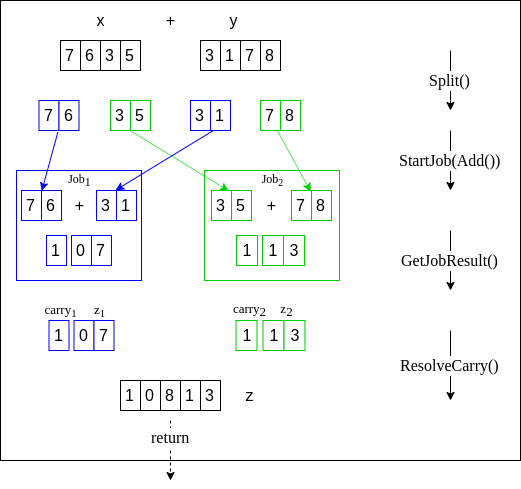
\includegraphics[width=0.75\textwidth]{resources/img/ch-3/add-example.png}
          \caption{Contoh Perhitungan Penjumlahan secara Paralel}
          \label{fig:add_par_example}
      \end{figure}

      Contoh perhitungan Pseudocode \ref{alg:parallel_add} untuk operasi $5235 + 2608$ dengan $\beta = 10$ dapat dilihat pada Gambar \ref{fig:add_par_example}. Pada contoh tersebut digunakan bilangan 4-word dengan basis 10. Sementara itu, jumlah job yang dibangkitkan adalah 2.

      % \todo[inline]{tambahin algoritma resolve carry juga, paralelin}

    \subsubsection{Perkalian} \label{sec:mul_parallel}

      Algoritma Karatsuba yang digunakan oleh OpenSSL merupakan sebuah algoritma rekursif. Paralelisasi fungsi yang menggunakan algoritma rekursif lebih mudah untuk dilakukan. Pemanggilan job secara paralel dilakukan dalam pemanggilan fungsi secara paralel.
      % \todo{tambahin citation ke buku}

      \citet{parallel_karatsuba_analysis} mengenalkan bahwa terdapat tiga strategi yang dapat dilakukan dalam batas pembagian job serta proses pembuatan job. Penelitian tersebut telah dibahas lebih lanjut  pada subbab \ref{sec:parallel_karatsuba}. Berdasarkan hasil penelitian yang dilakukan, strategi terbaik yang dapat dilakukan adalah menjalankan sebuah task pada job baru dan pada titik tertentu fungsi akan dijalankan secara sekuensial dan tidak secara paralel lagi. Berikut adalah pseudocode yang dapat digunakan untuk paralelisasi algoritma karatsuba.

      \begin{algorithm}
        \caption{Algoritma Perkalian Karatsuba Paralel}
        \begin{algorithmic}
          \Require{$A$ = [1..p], $B$ = [1..q] yang merepresentasikan Big Integer, $\beta$ adalah basis yang digunakan, $cutoff$ adalah batas maksimum Job yang dipanggil, $job_c$ adalah jumlah job saat ini yang diinisialisasi 1}
          \Statex
          \Function{MulKaratsubaParallel}{$A$, $B$, $\beta$, $cutoff$}
          \If{($p = 1$) or ($q = 1$)}
          \State \Return $A * B$
          \EndIf
          \Let{$mid$}{\Call{Floor}{\Call{Min}{$p, q$}/2}}
          \Let{$A_{low}, A_{high}$}{\Call{SplitIn}{$A, mid$}}
          \Let{$B_{low}, B_{high}$}{\Call{SplitIn}{$B, mid$}}
          \State
          \Let{$job_c$}{$job_c + 3$}
          \If{$job_c < cutoff$}
          \Let{$job_1$}{\Call{StartJob}{\Call{MulKaratsubaParallel}{$A_{low}, B_{low}$}}}
          \Let{$C_0$}{\Call{GetJobResult}{$job$}}

          \Let{$job_2$}{\Call{StartJob}{\Call{MulKaratsubaParallel}{($A_{low} + A_{high}$), ($B_{low} + B_{high}$)}}}
          \Let{$C_0$}{\Call{GetJobResult}{$job$}}

          \Let{$job_3$}{\Call{StartJob}{\Call{MulKaratsubaParallel}{$A_{high}, B_{high}$}}}
          \Let{$C_0$}{\Call{GetJobResult}{$job$}}
          \Else
          \Let{$C_0$}{\Call{MulKaratsuba}{$A_{low}, B_{low}$}}
          \Let{$C_1$}{\Call{MulKaratsuba}{($A_{low} + A_{high}$), ($B_{low} + B_{high}$)}}
          \Let{$C_2$}{\Call{MulKaratsuba}{$A_{high}, B_{high}$}}
          \EndIf

          \State
          \Let{$x$}{$C_2 * \beta ^ {mid * 2}$}
          \Let{$y$}{$(C_1 - C_2 - C_0) * \beta ^ {mid}$}

          \State \Return{$x + y + C_1$}
          \EndFunction
        \end{algorithmic}
      \end{algorithm}

      Algoritma perkalian panjang serta algoritma perkalian comba merupakan algoritma yang berbasis proses iterasi pada sebuah array. Dengan demikian, metode paralelisasi yang dapat digunakan mirip dengan proses paralelisasi untuk fungsi penjumlahan dan pengurangan pada subbab \ref{sec:add_sub_parallel}. Array dibagi menjadi beberapa subarray yang akan dikomputasi oleh sebuah job secara paralel. Pseudocode yang dapat digunakan untuk paralelisasi algoritma dapat dilihat pada pseudocode \ref{alg:mul_parallel}.

      \begin{algorithm}
        \caption{Algoritma Perkalian Panjang Paralel}
        \label{alg:mul_parallel}
        \begin{algorithmic}[1]
          \Require{$A$ = [1..p], $B$ = [1..q] yang merepresentasikan Big Integer, $\beta$ adalah basis yang digunakan representasi Big Integer, $num$ adalah jumlah job yang akan dipanggil}
          \Statex
          \Function{MulParallel}{$A$, $B$, $\beta$, $num$}
          \Let{C}{\Call{NewArray}{p+q}}
          \For{$i \gets 1$, $i \gets i + 1$ to $p$}
          \Let{$carry$}{0}
          \Let{$B_{chunks}$}{\Call{Split}{$B$, $num$}}
          \Let{$tmp\_result\_arr$}{\Call{NewArray}{$n$}}
          \ForAll{$i$, $j$ in $x_{chunks}$, $y_{chunks}$}
          \Let{$job$}{\Call{StartJob}{\Call{Mul}{$A$,$B_{chunks}$}}}
          \Let{$res$, $carry$}{\Call{GetJobResult}{$job$}}
          \State \Call{Append}{($res$, $carry$), $tmp\_result\_arr$}
          \EndFor
          \Call{ResolveCarry}{$tmp\_result\_arr$}
          \Let{$C[j + q]$}{$carry$}
          \EndFor
          \State \Return{$C$}
          \EndFunction
        \end{algorithmic}
      \end{algorithm}

    \subsubsection{Pembagian}\label{sec:div_parallel}
      Algoritma pembagian panjang yang digunakan OpenSSL tidak bisa dijalankan secara paralel mengingat setiap iterasi pencarian quotient membutuhkan nilai yang telah diupdate dari langkah sebelumnya. Namun, terdapat beberapa algoritma yang dapat membantu langkah pemilihan quotient pada baris ke-9 di pseudocode \ref{alg:long_div}. \citet{parallel_short_div_emmart} dan \citet{parallel_short_div_takahashi} telah melakukan penelitian mengenai pembagian \textit{multiple-precision big integer} terhadap bilangan \textit{single-word}.

      Ide dasar dari paralelisasi pemilihan quotient berdasarkan dari kebutuhan komputasi yang tinggi dari proses pemilihan quotient tersebut. Komputasi lain yang membutuhkan komputasi besar adalah perkalian pada pada langkah ke-11 di pseudocode \ref{alg:long_div}, namun proses perkalian dapat menggunakan algoritma perkalian paralel seperti yang telah dibahas pada subbab \ref{sec:mul_parallel}.

      % \begin{algorithm}
      %   \caption{Algoritma pemilihan quotient paralel}
      %   \label{alg:div_quotient_paralel}
      %   \begin{algorithmic}
      %     \Require{$A$ = [1..p] yang merepresentasikan Big Integer, $w$ adalah single-word integer, $\beta$ adalah basis yang digunakan representasi Big Integer}
      %     \Statex
      %     \Function{QuotientSelection}{$A, w, \beta$}
      %
      %     \EndFunction
      %   \end{algorithmic}
      % \end{algorithm}
